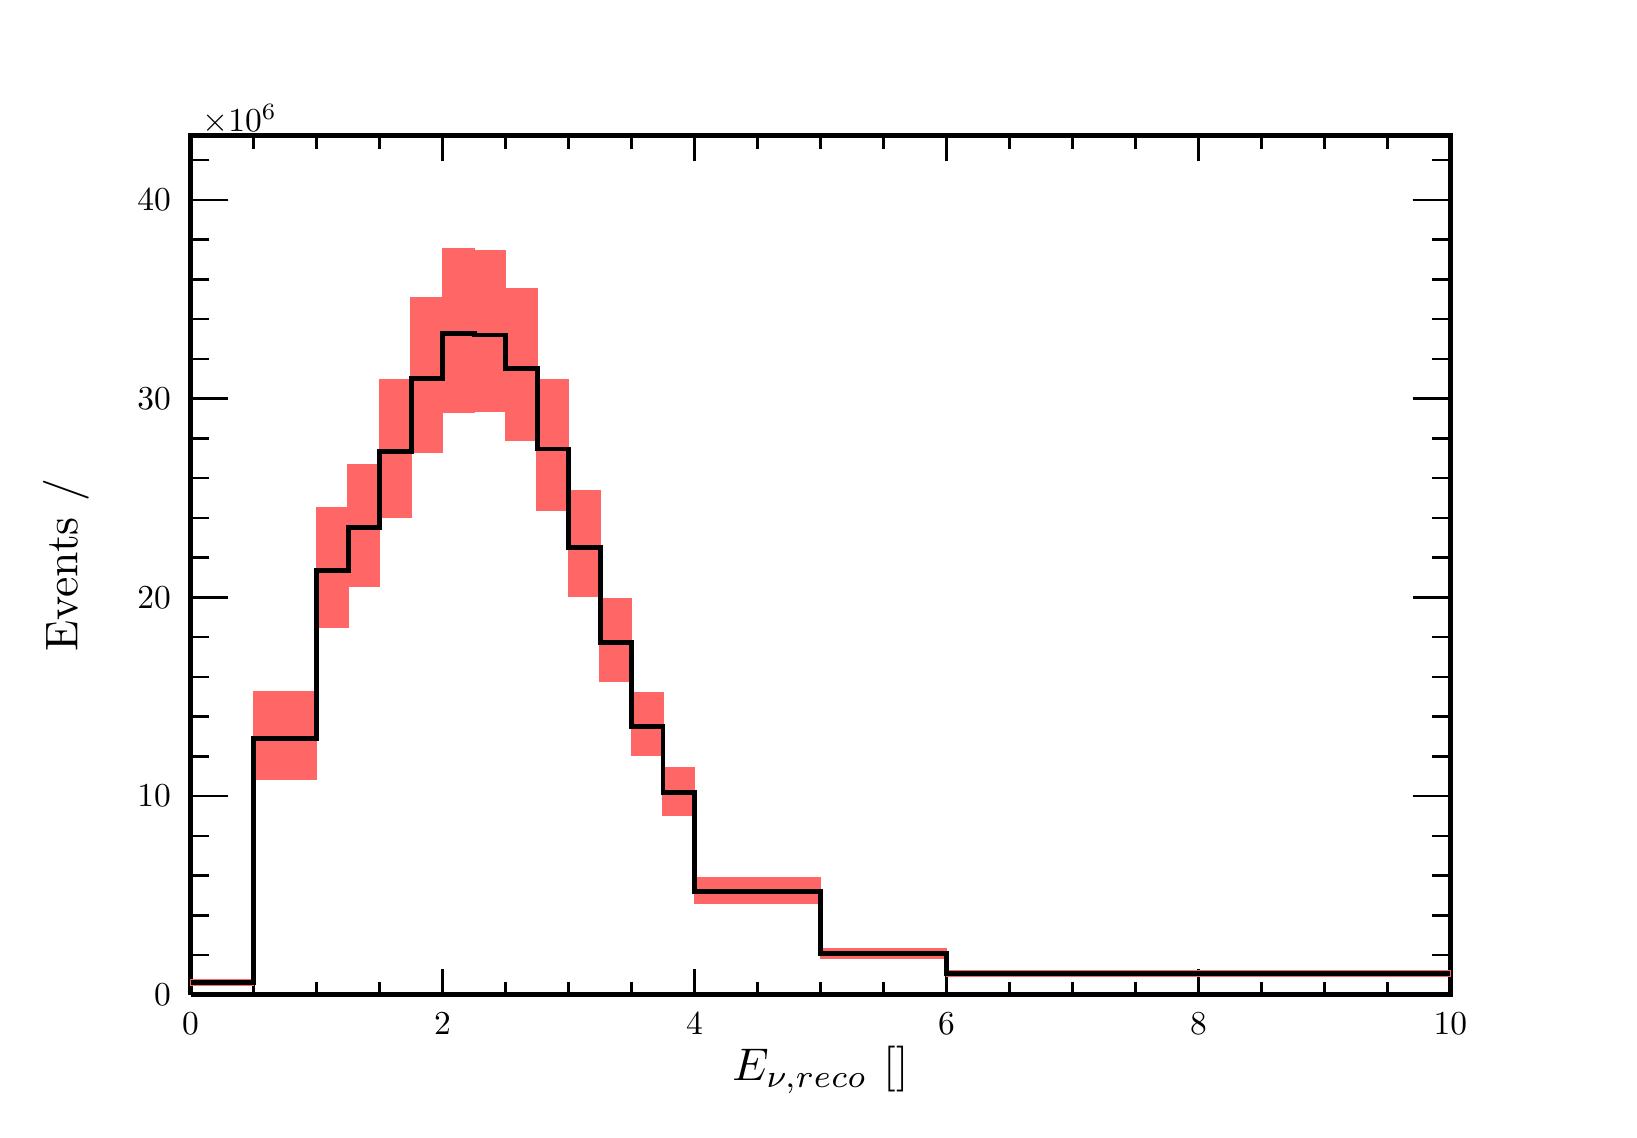
\begin{tikzpicture}
\pgfdeclareplotmark{cross} {
\pgfpathmoveto{\pgfpoint{-0.3\pgfplotmarksize}{\pgfplotmarksize}}
\pgfpathlineto{\pgfpoint{+0.3\pgfplotmarksize}{\pgfplotmarksize}}
\pgfpathlineto{\pgfpoint{+0.3\pgfplotmarksize}{0.3\pgfplotmarksize}}
\pgfpathlineto{\pgfpoint{+1\pgfplotmarksize}{0.3\pgfplotmarksize}}
\pgfpathlineto{\pgfpoint{+1\pgfplotmarksize}{-0.3\pgfplotmarksize}}
\pgfpathlineto{\pgfpoint{+0.3\pgfplotmarksize}{-0.3\pgfplotmarksize}}
\pgfpathlineto{\pgfpoint{+0.3\pgfplotmarksize}{-1.\pgfplotmarksize}}
\pgfpathlineto{\pgfpoint{-0.3\pgfplotmarksize}{-1.\pgfplotmarksize}}
\pgfpathlineto{\pgfpoint{-0.3\pgfplotmarksize}{-0.3\pgfplotmarksize}}
\pgfpathlineto{\pgfpoint{-1.\pgfplotmarksize}{-0.3\pgfplotmarksize}}
\pgfpathlineto{\pgfpoint{-1.\pgfplotmarksize}{0.3\pgfplotmarksize}}
\pgfpathlineto{\pgfpoint{-0.3\pgfplotmarksize}{0.3\pgfplotmarksize}}
\pgfpathclose
\pgfusepathqstroke
}
\pgfdeclareplotmark{cross*} {
\pgfpathmoveto{\pgfpoint{-0.3\pgfplotmarksize}{\pgfplotmarksize}}
\pgfpathlineto{\pgfpoint{+0.3\pgfplotmarksize}{\pgfplotmarksize}}
\pgfpathlineto{\pgfpoint{+0.3\pgfplotmarksize}{0.3\pgfplotmarksize}}
\pgfpathlineto{\pgfpoint{+1\pgfplotmarksize}{0.3\pgfplotmarksize}}
\pgfpathlineto{\pgfpoint{+1\pgfplotmarksize}{-0.3\pgfplotmarksize}}
\pgfpathlineto{\pgfpoint{+0.3\pgfplotmarksize}{-0.3\pgfplotmarksize}}
\pgfpathlineto{\pgfpoint{+0.3\pgfplotmarksize}{-1.\pgfplotmarksize}}
\pgfpathlineto{\pgfpoint{-0.3\pgfplotmarksize}{-1.\pgfplotmarksize}}
\pgfpathlineto{\pgfpoint{-0.3\pgfplotmarksize}{-0.3\pgfplotmarksize}}
\pgfpathlineto{\pgfpoint{-1.\pgfplotmarksize}{-0.3\pgfplotmarksize}}
\pgfpathlineto{\pgfpoint{-1.\pgfplotmarksize}{0.3\pgfplotmarksize}}
\pgfpathlineto{\pgfpoint{-0.3\pgfplotmarksize}{0.3\pgfplotmarksize}}
\pgfpathclose
\pgfusepathqfillstroke
}
\pgfdeclareplotmark{newstar} {
\pgfpathmoveto{\pgfqpoint{0pt}{\pgfplotmarksize}}
\pgfpathlineto{\pgfqpointpolar{44}{0.5\pgfplotmarksize}}
\pgfpathlineto{\pgfqpointpolar{18}{\pgfplotmarksize}}
\pgfpathlineto{\pgfqpointpolar{-20}{0.5\pgfplotmarksize}}
\pgfpathlineto{\pgfqpointpolar{-54}{\pgfplotmarksize}}
\pgfpathlineto{\pgfqpointpolar{-90}{0.5\pgfplotmarksize}}
\pgfpathlineto{\pgfqpointpolar{234}{\pgfplotmarksize}}
\pgfpathlineto{\pgfqpointpolar{198}{0.5\pgfplotmarksize}}
\pgfpathlineto{\pgfqpointpolar{162}{\pgfplotmarksize}}
\pgfpathlineto{\pgfqpointpolar{134}{0.5\pgfplotmarksize}}
\pgfpathclose
\pgfusepathqstroke
}
\pgfdeclareplotmark{newstar*} {
\pgfpathmoveto{\pgfqpoint{0pt}{\pgfplotmarksize}}
\pgfpathlineto{\pgfqpointpolar{44}{0.5\pgfplotmarksize}}
\pgfpathlineto{\pgfqpointpolar{18}{\pgfplotmarksize}}
\pgfpathlineto{\pgfqpointpolar{-20}{0.5\pgfplotmarksize}}
\pgfpathlineto{\pgfqpointpolar{-54}{\pgfplotmarksize}}
\pgfpathlineto{\pgfqpointpolar{-90}{0.5\pgfplotmarksize}}
\pgfpathlineto{\pgfqpointpolar{234}{\pgfplotmarksize}}
\pgfpathlineto{\pgfqpointpolar{198}{0.5\pgfplotmarksize}}
\pgfpathlineto{\pgfqpointpolar{162}{\pgfplotmarksize}}
\pgfpathlineto{\pgfqpointpolar{134}{0.5\pgfplotmarksize}}
\pgfpathclose
\pgfusepathqfillstroke
}
\definecolor{c}{rgb}{0.999,0.999,0.999};
\draw [color=c, fill=c] (0,0) rectangle (20,13.639);
\draw [color=c, fill=c] (2,1.3639) rectangle (18,12.2751);
\definecolor{c}{rgb}{0,0,0};
\draw [c,line width=1.8] (2,1.3639) -- (2,12.2751) -- (18,12.2751) -- (18,1.3639) -- (2,1.3639);
\definecolor{c}{rgb}{0.999,0.999,0.999};
\draw [color=c, fill=c] (2,1.3639) rectangle (18,12.2751);
\definecolor{c}{rgb}{0,0,0};
\draw [c,line width=1.8] (2,1.3639) -- (2,12.2751) -- (18,12.2751) -- (18,1.3639) -- (2,1.3639);
\draw [c,line width=1.8] (2,1.51493) -- (2.8,1.51493) -- (2.8,4.62211) -- (3.6,4.62211) -- (3.6,6.74706) -- (4,6.74706) -- (4,7.2923) -- (4.4,7.2923) -- (4.4,8.26899) -- (4.8,8.26899) -- (4.8,9.19574) -- (5.2,9.19574) -- (5.2,9.75711) --
 (5.6,9.75711) -- (5.6,9.74279) -- (6,9.74279) -- (6,9.31443) -- (6.4,9.31443) -- (6.4,8.29504) -- (6.8,8.29504) -- (6.8,7.04862) -- (7.2,7.04862) -- (7.2,5.83584) -- (7.6,5.83584) -- (7.6,4.77677) -- (8,4.77677) -- (8,3.92868) -- (8.4,3.92868) --
 (8.4,2.68015) -- (10,2.68015) -- (10,1.88528) -- (11.6,1.88528) -- (11.6,1.63144) -- (18,1.63144);
\draw [c,line width=0.9] (2,1.3639) -- (18,1.3639);
\draw [c,line width=0.9] (2,1.69123) -- (2,1.3639);
\draw [c,line width=0.9] (2.8,1.52756) -- (2.8,1.3639);
\draw [c,line width=0.9] (3.6,1.52756) -- (3.6,1.3639);
\draw [c,line width=0.9] (4.4,1.52756) -- (4.4,1.3639);
\draw [c,line width=0.9] (5.2,1.69123) -- (5.2,1.3639);
\draw [c,line width=0.9] (6,1.52756) -- (6,1.3639);
\draw [c,line width=0.9] (6.8,1.52756) -- (6.8,1.3639);
\draw [c,line width=0.9] (7.6,1.52756) -- (7.6,1.3639);
\draw [c,line width=0.9] (8.4,1.69123) -- (8.4,1.3639);
\draw [c,line width=0.9] (9.2,1.52756) -- (9.2,1.3639);
\draw [c,line width=0.9] (10,1.52756) -- (10,1.3639);
\draw [c,line width=0.9] (10.8,1.52756) -- (10.8,1.3639);
\draw [c,line width=0.9] (11.6,1.69123) -- (11.6,1.3639);
\draw [c,line width=0.9] (12.4,1.52756) -- (12.4,1.3639);
\draw [c,line width=0.9] (13.2,1.52756) -- (13.2,1.3639);
\draw [c,line width=0.9] (14,1.52756) -- (14,1.3639);
\draw [c,line width=0.9] (14.8,1.69123) -- (14.8,1.3639);
\draw [c,line width=0.9] (15.6,1.52756) -- (15.6,1.3639);
\draw [c,line width=0.9] (16.4,1.52756) -- (16.4,1.3639);
\draw [c,line width=0.9] (17.2,1.52756) -- (17.2,1.3639);
\draw [c,line width=0.9] (18,1.69123) -- (18,1.3639);
\draw [anchor=base] (2,0.859255) node[scale=1.20912, color=c, rotate=0]{0};
\draw [anchor=base] (5.2,0.859255) node[scale=1.20912, color=c, rotate=0]{2};
\draw [anchor=base] (8.4,0.859255) node[scale=1.20912, color=c, rotate=0]{4};
\draw [anchor=base] (11.6,0.859255) node[scale=1.20912, color=c, rotate=0]{6};
\draw [anchor=base] (14.8,0.859255) node[scale=1.20912, color=c, rotate=0]{8};
\draw [anchor=base] (18,0.859255) node[scale=1.20912, color=c, rotate=0]{10};
\draw (10,0.403714) node[scale=1.65459, color=c, rotate=0]{$E_{\nu, \text{reco}}$ [\si{\GeV}]};
\draw [c,line width=0.9] (2,12.2751) -- (18,12.2751);
\draw [c,line width=0.9] (2,11.9477) -- (2,12.2751);
\draw [c,line width=0.9] (2.8,12.1114) -- (2.8,12.2751);
\draw [c,line width=0.9] (3.6,12.1114) -- (3.6,12.2751);
\draw [c,line width=0.9] (4.4,12.1114) -- (4.4,12.2751);
\draw [c,line width=0.9] (5.2,11.9477) -- (5.2,12.2751);
\draw [c,line width=0.9] (6,12.1114) -- (6,12.2751);
\draw [c,line width=0.9] (6.8,12.1114) -- (6.8,12.2751);
\draw [c,line width=0.9] (7.6,12.1114) -- (7.6,12.2751);
\draw [c,line width=0.9] (8.4,11.9477) -- (8.4,12.2751);
\draw [c,line width=0.9] (9.2,12.1114) -- (9.2,12.2751);
\draw [c,line width=0.9] (10,12.1114) -- (10,12.2751);
\draw [c,line width=0.9] (10.8,12.1114) -- (10.8,12.2751);
\draw [c,line width=0.9] (11.6,11.9477) -- (11.6,12.2751);
\draw [c,line width=0.9] (12.4,12.1114) -- (12.4,12.2751);
\draw [c,line width=0.9] (13.2,12.1114) -- (13.2,12.2751);
\draw [c,line width=0.9] (14,12.1114) -- (14,12.2751);
\draw [c,line width=0.9] (14.8,11.9477) -- (14.8,12.2751);
\draw [c,line width=0.9] (15.6,12.1114) -- (15.6,12.2751);
\draw [c,line width=0.9] (16.4,12.1114) -- (16.4,12.2751);
\draw [c,line width=0.9] (17.2,12.1114) -- (17.2,12.2751);
\draw [c,line width=0.9] (18,11.9477) -- (18,12.2751);
\draw [c,line width=0.9] (2,1.3639) -- (2,12.2751);
\draw [c,line width=0.9] (2.48,1.3639) -- (2,1.3639);
\draw [c,line width=0.9] (2.24,1.86859) -- (2,1.86859);
\draw [c,line width=0.9] (2.24,2.37329) -- (2,2.37329);
\draw [c,line width=0.9] (2.24,2.87799) -- (2,2.87799);
\draw [c,line width=0.9] (2.24,3.38268) -- (2,3.38268);
\draw [c,line width=0.9] (2.48,3.88738) -- (2,3.88738);
\draw [c,line width=0.9] (2.24,4.39208) -- (2,4.39208);
\draw [c,line width=0.9] (2.24,4.89677) -- (2,4.89677);
\draw [c,line width=0.9] (2.24,5.40147) -- (2,5.40147);
\draw [c,line width=0.9] (2.24,5.90617) -- (2,5.90617);
\draw [c,line width=0.9] (2.48,6.41086) -- (2,6.41086);
\draw [c,line width=0.9] (2.24,6.91556) -- (2,6.91556);
\draw [c,line width=0.9] (2.24,7.42026) -- (2,7.42026);
\draw [c,line width=0.9] (2.24,7.92495) -- (2,7.92495);
\draw [c,line width=0.9] (2.24,8.42965) -- (2,8.42965);
\draw [c,line width=0.9] (2.48,8.93435) -- (2,8.93435);
\draw [c,line width=0.9] (2.24,9.43904) -- (2,9.43904);
\draw [c,line width=0.9] (2.24,9.94374) -- (2,9.94374);
\draw [c,line width=0.9] (2.24,10.4484) -- (2,10.4484);
\draw [c,line width=0.9] (2.24,10.9531) -- (2,10.9531);
\draw [c,line width=0.9] (2.48,11.4578) -- (2,11.4578);
\draw [c,line width=0.9] (2.48,11.4578) -- (2,11.4578);
\draw [c,line width=0.9] (2.24,11.9625) -- (2,11.9625);
\draw [anchor= east] (1.9,1.3639) node[scale=1.20912, color=c, rotate=0]{0};
\draw [anchor= east] (1.9,3.88738) node[scale=1.20912, color=c, rotate=0]{10};
\draw [anchor= east] (1.9,6.41086) node[scale=1.20912, color=c, rotate=0]{20};
\draw [anchor= east] (1.9,8.93435) node[scale=1.20912, color=c, rotate=0]{30};
\draw [anchor= east] (1.9,11.4578) node[scale=1.20912, color=c, rotate=0]{40};
\draw [anchor=base west] (2,12.3296) node[scale=1.20912, color=c, rotate=0]{$\times10^{6}$};
\draw (0.416,6.81948) node[scale=1.65459, color=c, rotate=90]{Events / \si{\GeV}};
\draw [c,line width=0.9] (18,1.3639) -- (18,12.2751);
\draw [c,line width=0.9] (17.52,1.3639) -- (18,1.3639);
\draw [c,line width=0.9] (17.76,1.86859) -- (18,1.86859);
\draw [c,line width=0.9] (17.76,2.37329) -- (18,2.37329);
\draw [c,line width=0.9] (17.76,2.87799) -- (18,2.87799);
\draw [c,line width=0.9] (17.76,3.38268) -- (18,3.38268);
\draw [c,line width=0.9] (17.52,3.88738) -- (18,3.88738);
\draw [c,line width=0.9] (17.76,4.39208) -- (18,4.39208);
\draw [c,line width=0.9] (17.76,4.89677) -- (18,4.89677);
\draw [c,line width=0.9] (17.76,5.40147) -- (18,5.40147);
\draw [c,line width=0.9] (17.76,5.90617) -- (18,5.90617);
\draw [c,line width=0.9] (17.52,6.41086) -- (18,6.41086);
\draw [c,line width=0.9] (17.76,6.91556) -- (18,6.91556);
\draw [c,line width=0.9] (17.76,7.42026) -- (18,7.42026);
\draw [c,line width=0.9] (17.76,7.92495) -- (18,7.92495);
\draw [c,line width=0.9] (17.76,8.42965) -- (18,8.42965);
\draw [c,line width=0.9] (17.52,8.93435) -- (18,8.93435);
\draw [c,line width=0.9] (17.76,9.43904) -- (18,9.43904);
\draw [c,line width=0.9] (17.76,9.94374) -- (18,9.94374);
\draw [c,line width=0.9] (17.76,10.4484) -- (18,10.4484);
\draw [c,line width=0.9] (17.76,10.9531) -- (18,10.9531);
\draw [c,line width=0.9] (17.52,11.4578) -- (18,11.4578);
\draw [c,line width=0.9] (17.52,11.4578) -- (18,11.4578);
\draw [c,line width=0.9] (17.76,11.9625) -- (18,11.9625);
\definecolor{c}{rgb}{1,0.4,0.4};
\draw [color=c, fill=c] (2,1.48034) rectangle (2.8,1.55148);
\draw [color=c, fill=c] (2.8,4.10305) rectangle (3.6,5.21699);
\draw [color=c, fill=c] (3.6,6.03199) rectangle (4,7.54785);
\draw [color=c, fill=c] (4,6.54917) rectangle (4.4,8.10234);
\draw [color=c, fill=c] (4.4,7.42277) rectangle (4.8,9.17979);
\draw [color=c, fill=c] (4.8,8.25416) rectangle (5.2,10.2134);
\draw [color=c, fill=c] (5.2,8.76516) rectangle (5.6,10.8389);
\draw [color=c, fill=c] (5.6,8.76627) rectangle (6,10.8176);
\draw [color=c, fill=c] (6,8.39864) rectangle (6.4,10.3341);
\draw [color=c, fill=c] (6.4,7.51232) rectangle (6.8,9.1725);
\draw [color=c, fill=c] (6.8,6.41696) rectangle (7.2,7.76296);
\draw [color=c, fill=c] (7.2,5.34104) rectangle (7.6,6.40042);
\draw [color=c, fill=c] (7.6,4.40155) rectangle (8,5.20583);
\draw [color=c, fill=c] (8,3.64328) rectangle (8.4,4.25281);
\draw [color=c, fill=c] (8.4,2.52743) rectangle (10,2.85207);
\draw [color=c, fill=c] (10,1.82219) rectangle (11.6,1.95458);
\draw [color=c, fill=c] (11.6,1.59807) rectangle (18,1.66732);
\definecolor{c}{rgb}{0,0,0};
\draw [c,line width=1.8] (2,1.51493) -- (2.8,1.51493) -- (2.8,4.62211) -- (3.6,4.62211) -- (3.6,6.74706) -- (4,6.74706) -- (4,7.2923) -- (4.4,7.2923) -- (4.4,8.26899) -- (4.8,8.26899) -- (4.8,9.19574) -- (5.2,9.19574) -- (5.2,9.75711) --
 (5.6,9.75711) -- (5.6,9.74279) -- (6,9.74279) -- (6,9.31443) -- (6.4,9.31443) -- (6.4,8.29504) -- (6.8,8.29504) -- (6.8,7.04862) -- (7.2,7.04862) -- (7.2,5.83584) -- (7.6,5.83584) -- (7.6,4.77677) -- (8,4.77677) -- (8,3.92868) -- (8.4,3.92868) --
 (8.4,2.68015) -- (10,2.68015) -- (10,1.88528) -- (11.6,1.88528) -- (11.6,1.63144) -- (18,1.63144);
\end{tikzpicture}
